\section{Poor Man's Scaling}

We first quote some results from Anderson's scaling method, as it is instructive to see where the qualitative conclusion of increasing coupling comes from, as well as why its successive renormalization means it fails in the low temperature regime.


\subsection{The Scattering \texorpdfstring{$T$}{T}-Matrix}

The way this was calculated was via the scattering $T$-matrix. This is very similar to the born series, which looks like

\begin{equation}
  \psi = \psi_0 + \int\; gV\psi_0 + \int\int\; gVgV\psi_0 + \int\int\int\; gVgVgV\psi_0 + \ldots.
\end{equation}

This is a way to achieve approximate scattering results via a Green's function $g$ and a potential $V$. The $T$-matrix representing scattering of an electron from an initial state $\ket{\vv{k}}$ to final state $\ket{\vv{k}'}$ looks like, to second order:

\begin{equation}
  T_{\vv{k},\vv{k}}(\omega) = V_{\vv{k}',\vv{k}} + V_{\vv{k}',\vv{q}} G_0(\omega, \vv{q})T(\omega).
\end{equation}

\begin{figure}
  \centering
  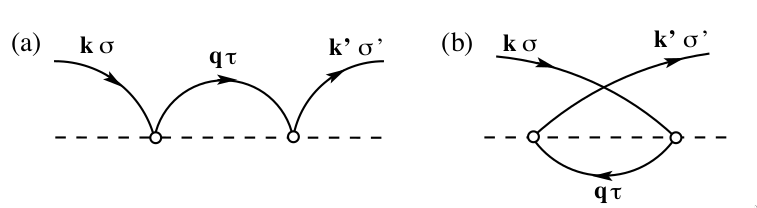
\includegraphics[width=0.6\linewidth]{./gfx/poormans-feynman.png}
  \caption{Feynman diagrams describing the spin scattering of the impurity electron and conduction electron used to calculate the $T$-matrix elements.}
  \label{fig:2-poormans-diagrams}
\end{figure}

Feynman diagrams for this process are given in Fig.~\ref{fig:2-poormans-diagrams}. Here, the ``potential'' term $V$ is related to the coupling; hence, to second order, what we have upon doing this calculation is the effective renormalization of the potential, which corresponds to the coupling $J$:

\begin{equation}
  \hat{V} \rightarrow \hat{V}' = \hat{V} + \hat{V} \frac{1}{\omega - \hat{H}_0}\hat{V},\label{eq:2-poormans-v-renorm}
\end{equation}

where

\begin{equation}
  G_0 = \frac{1}{\omega - \hat{H}_0}
\end{equation}

is the Green's function. At this point, I will now quote results, as it would have been far too challenging to exhaustively study this as well as the NRG. As Eq.~\eqref{eq:2-poormans-v-renorm} implies, we have a normalization of the coupling like $J_\alpha \rightarrow J_\alpha + \delta J_\alpha$, where $\alpha = \pm,z$. Anderson found that the forms of the $\delta J_\alpha$s look like:

\begin{align}
  \delta J_z &= -J_\pm^2 \rho \abs{\delta\Lambda} \left[ \frac{1}{\omega - \Lambda + \epsilon_k} + \frac{1}{\omega - \Lambda - \epsilon_{k'}} \right], \\
  \delta J_\pm &= -J_z J_\pm \rho \abs{\delta\Lambda} \left[ \frac{1}{\omega - \Lambda + \epsilon_k} + \frac{1}{\omega - \Lambda - \epsilon_{k'}} \right].
\end{align}

Introducing dimensionless coupling constants $g_\alpha \equiv \rho J_\alpha$, we are able to find renormalization flow equations that look like:

\begin{align}
  \diff{g_z}{\ln\Lambda} &= -2g_\pm^2 + \mathcal{O}(g^3), \\
  \diff{g_\pm}{\ln\Lambda} &= -2g_z g_\pm + \mathcal{O}(g^3).
\end{align}


\subsection{Qualitative Conclusions}

There is one important case to consider: the antiferromagnetic one. In this case, the couplings are positive, so the overall minus remains. This signifies that as the energy decreases, the coupling will increase without bound. This was one main result from this method; however, the other was that the $T$-matrix formalism, i.e. expansion up to second order, is valid insofar as the coupling (represented by $V$) remains small. However, it clearly shoots up to infinity, making this method incompatible with the very low-energy regime.

Despite this failure, the increasing coupling was not disregarded. The thought upon this discovery was that there was some sort of bound state forming between the impurity and the conduction electrons, which was made possible by the increasingly large coupling. In the following section, we will explore some variational methods applied to this problem, and we will find that this bound state is precisely the one that is most likely, and we will gain some more of a qualitative understanding of what is happening at low energy.



%%% Local Variables:
%%% mode: LaTeX
%%% TeX-master: "../project"
%%% End:
